\chapter{System Modeling}
With the given setup being described, it is necessary to study its natural behavior in more detail by deriving a model of this system. This chapter shows the process used to put up this model.

A mechanical drawing of the Cubli showing angles and coordinate system conventions is seen in \figref{cubliMechanical}. A two-dimensional global coordinate system is chosen with its origin on the pivot point of the frame. Moreover, the positive direction of the angles is chosen to be clockwise.

\begin{figure}[H]
 \centering
 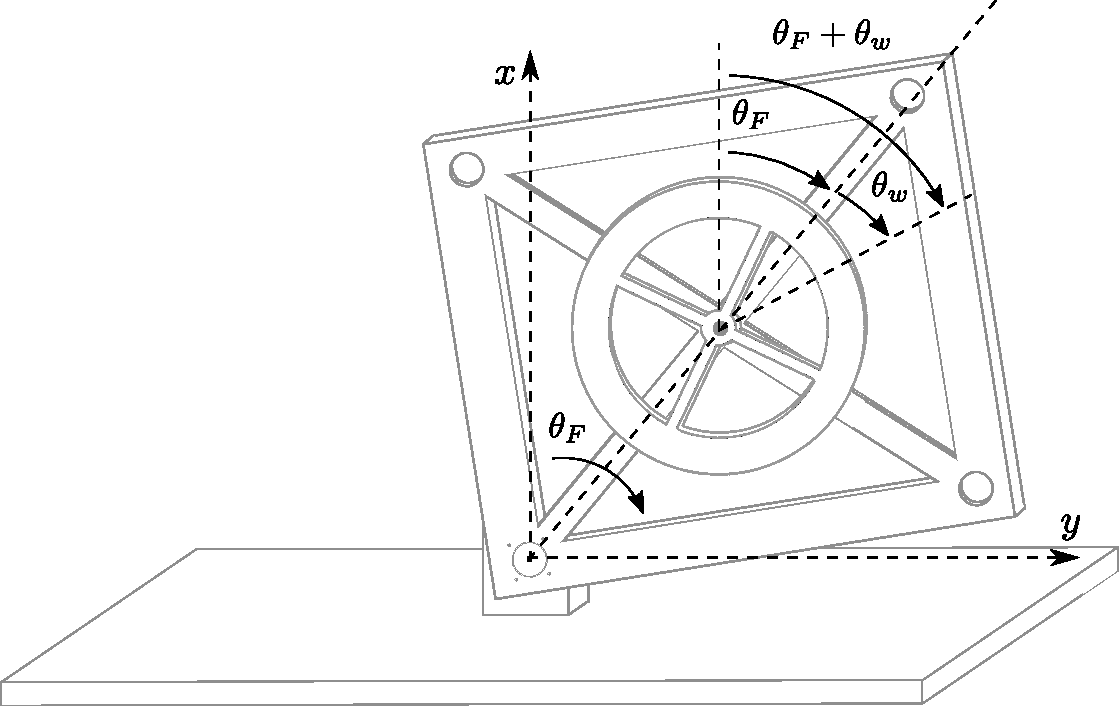
\includegraphics[scale=0.6]{figures/mechanicalSystem}
 \caption{Mechanical drawing of the Cubli, including coordinate system and angle conventions. Note that the x axis is pointing upwards.}
 \label{cubliMechanical}
\end{figure}

%As shown in \figref{cubliMechanical}, 
In next section, a complete model of the given setup is derived from Newton's Second Law of motion and rotation.